\documentclass[a4paper, 11pt]{article}
\usepackage[czech]{babel}
\usepackage[top=3cm, left=2cm, text={17cm, 24cm}]{geometry}
\usepackage[utf8]{inputenc}
\usepackage{times}
\usepackage{graphicx}
\usepackage{float}

\begin{document}

\begin{center}
\LARGE{Profiling protokol\\}
\end{center}

Program odchylka byl postupně spouštěň s 10, 100, 1000 vstupních hodnot s použitím profileru gprof. Níže jsou přiloženy screenshoty z výstupů gprof, ve kterém jsou údaje s názvy volaných funkcí, jejich počtu zavolání a časem strávených v nich.

\begin{figure}[h]
\centering
Pro zavolání programu s 10 vstupními hodnotami:\\
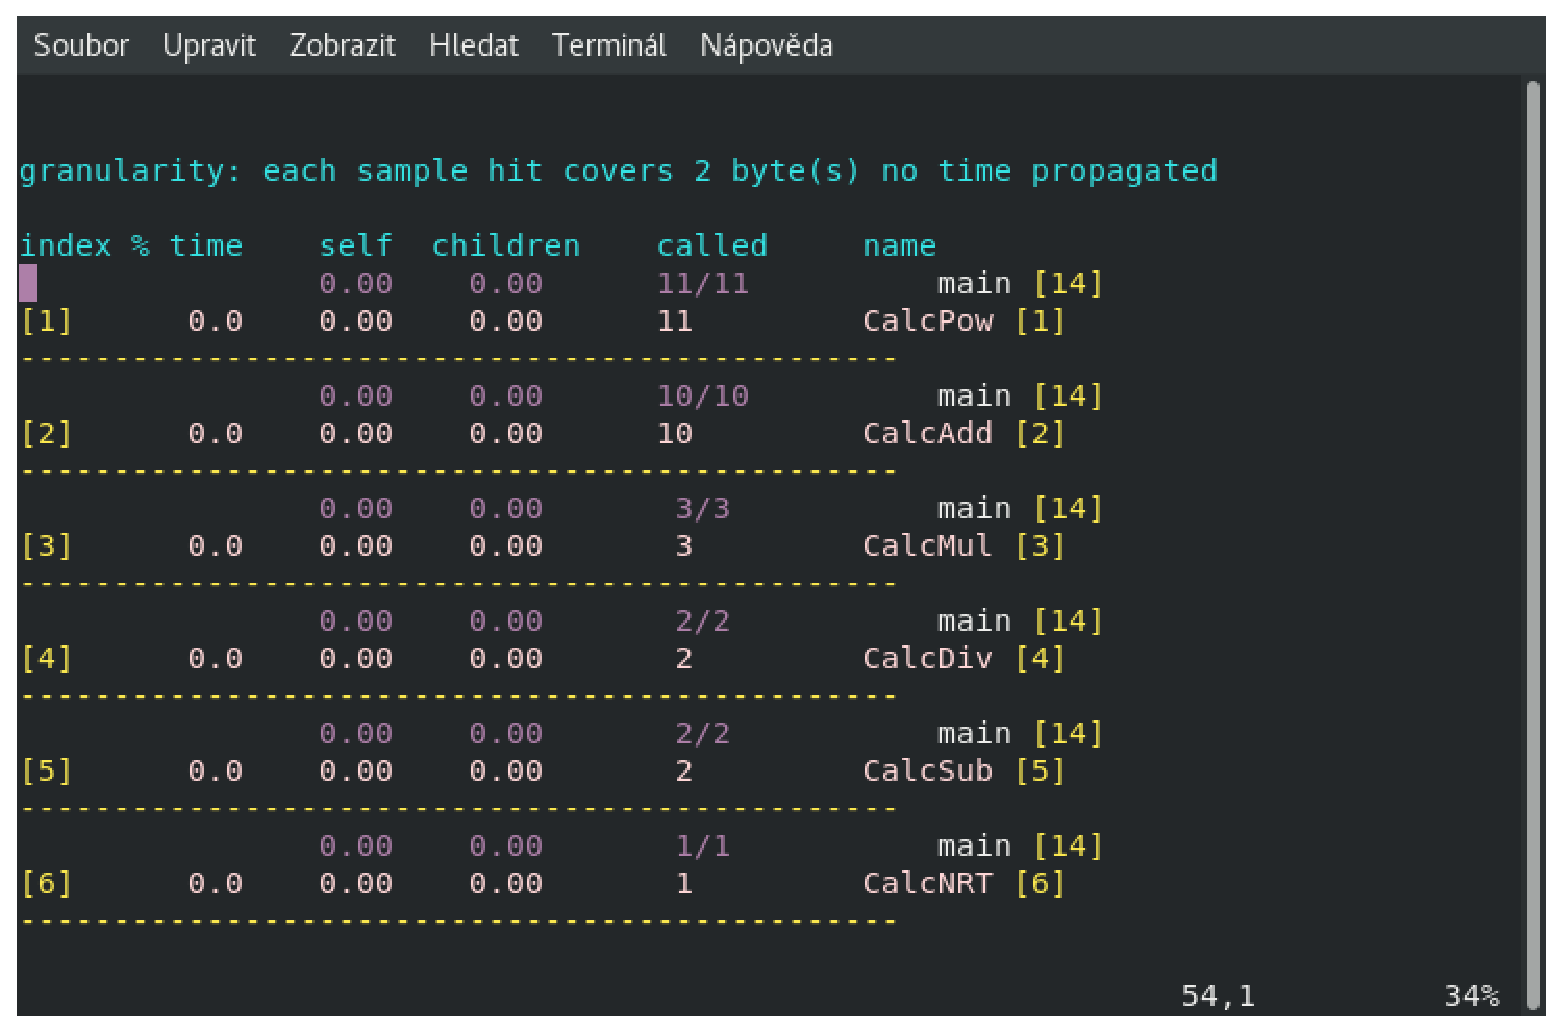
\includegraphics[scale=0.5]{10}\bigskip\\
Pro zavolání programu se 100 vstupních hodnot:\\
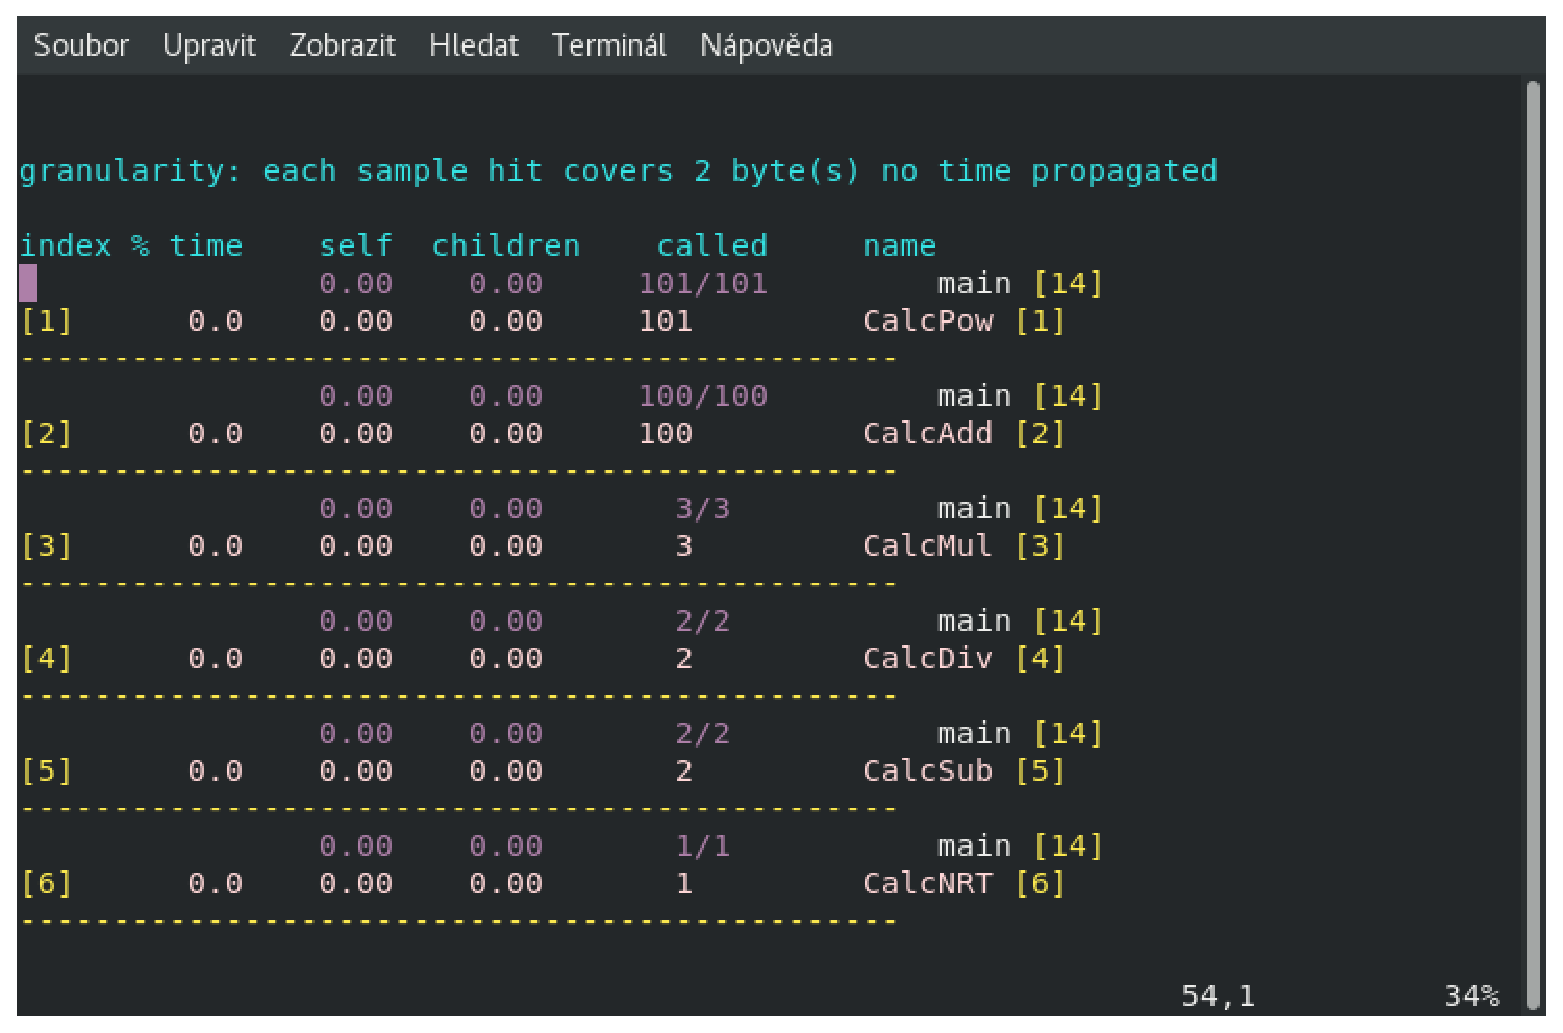
\includegraphics[scale=0.5]{100}\bigskip
\end{figure}

\begin{figure}[H]
\centering
Pro zavolání programu s 1000 vstupních hodnot:\\
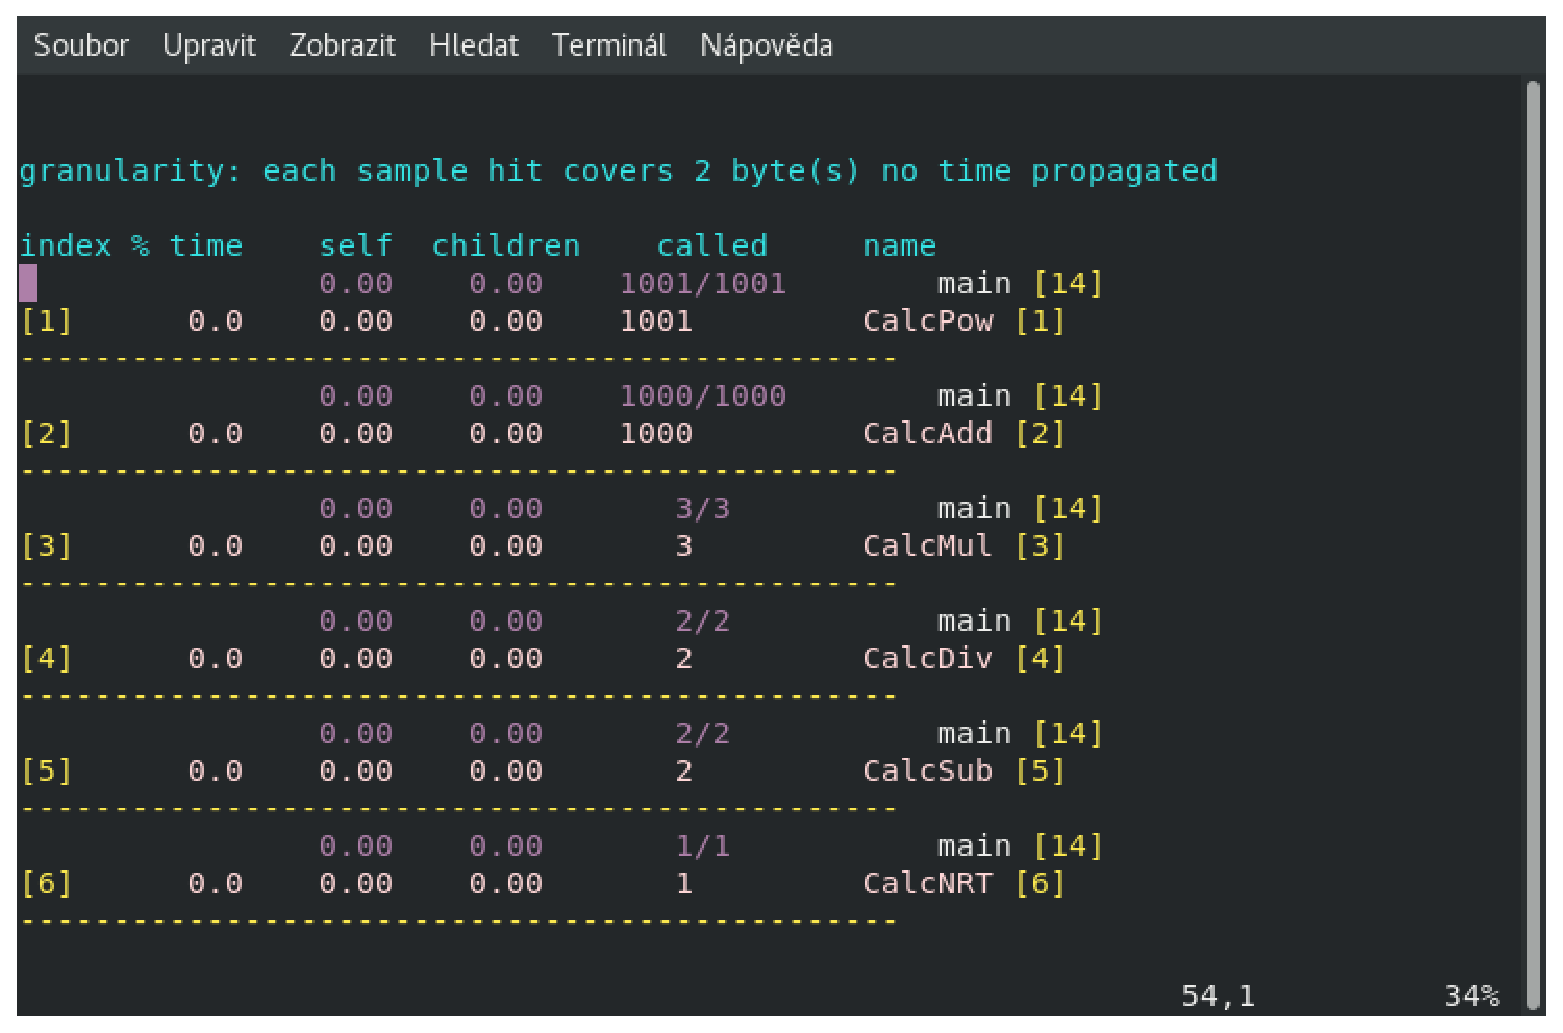
\includegraphics[scale=0.5]{1000}\bigskip
\end{figure}

\section*{Závěr}
Funkce probíhaly rychleji, než je vzorkovací čas profileru (0.1 s), tudíž nebyl schopný naměřit žádný čas.\par
Návrhy pro zrychlení programu:
\begin{itemize}
\item Realokování pole pro načítání prvků o více než jeden prvek (Sníží se počet volání realokací, ale vzniknou větší požadavky na paměť.)
\item Upravením početních operací ve vzorci na početní operace efektivnější pro procesor
\item Upravením vyhodnocovacích podmínek pro cykly a pro if rozhodování
\item Použítím méně přesných, ale rychlejších výpočtů např. pro výpočet logaritmů
\end{itemize}

\vfill
\today \hfill Patrik Polášek

\end{document}
